\documentclass{IEEEcsmag}
%DIF LATEXDIFF DIFFERENCE FILE
%DIF DEL original-submission/Fast_ParaView.tex      Mon Mar  4 09:38:15 2024
%DIF ADD original-submission/../Fast_ParaView.tex   Wed Mar  6 16:14:49 2024


\usepackage[colorlinks,urlcolor=blue,linkcolor=blue,citecolor=blue]{hyperref}

\usepackage{upmath}

\jvol{XX}
\jnum{XX}
\paper{8}
\jmonth{May/June}
\jname{IT Professional}
%DIF 13c13
%DIF < \pubyear{2021}
%DIF -------
\pubyear{2024} %DIF > 
%DIF -------

\newtheorem{theorem}{Theorem}
\newtheorem{lemma}{Lemma}


\setcounter{secnumdepth}{0}

\graphicspath{{pics/}}

\hyphenation{Para-View}

\usepackage{color}
\newcommand*{\fix}[1]{\textbf{\emph{\textcolor{red}{#1}}}}

%DIF 28c28-29
%DIF < \usepackage{subcaption}
%DIF -------
\definecolor{km}{RGB}{105, 41, 197} %DIF > 
\definecolor{fs}{RGB}{17, 146, 233} %DIF > 
%DIF -------

%DIF 30a31-38
\newcommand*{\km}[1]{\textcolor{km}{\emph{\textbf{#1} -- KM}}} %DIF > 
\newcommand*{\fs}[1]{\textcolor{fs}{\emph{\textbf{#1} -- FS}}} %DIF > 
 %DIF > 
\usepackage{booktabs} %DIF > 
\usepackage{dblfloatfix} %DIF > 
\usepackage{multirow} %DIF > 
\usepackage{paralist} %DIF > 
\usepackage{subcaption} %DIF > 
%DIF -------
\usepackage{xspace}

\newcommand*{\colormap}[1]{\textsl{#1}\xspace}
\newcommand*{\huewheel}{\colormap{Hue Wheel}}
\newcommand*{\coolwarm}{\colormap{Cool to Warm}}
\newcommand*{\blueorange}{\colormap{Blue-Orange Diverging}}
\newcommand*{\fast}{\colormap{Fast}}
\newcommand*{\turbo}{\colormap{Turbo}}
\newcommand*{\extendedcoolwarm}{\colormap{Extended Cool Warm}} %DIF > 
%DIF PREAMBLE EXTENSION ADDED BY LATEXDIFF
%DIF UNDERLINE PREAMBLE %DIF PREAMBLE
\RequirePackage[normalem]{ulem} %DIF PREAMBLE
\RequirePackage{color}\definecolor{RED}{rgb}{1,0,0}\definecolor{BLUE}{rgb}{0,0,1} %DIF PREAMBLE
\providecommand{\DIFaddtex}[1]{{\protect\color{blue}\uwave{#1}}} %DIF PREAMBLE
\providecommand{\DIFdeltex}[1]{{\protect\color{red}\sout{#1}}}                      %DIF PREAMBLE
%DIF SAFE PREAMBLE %DIF PREAMBLE
\providecommand{\DIFaddbegin}{} %DIF PREAMBLE
\providecommand{\DIFaddend}{} %DIF PREAMBLE
\providecommand{\DIFdelbegin}{} %DIF PREAMBLE
\providecommand{\DIFdelend}{} %DIF PREAMBLE
\providecommand{\DIFmodbegin}{} %DIF PREAMBLE
\providecommand{\DIFmodend}{} %DIF PREAMBLE
%DIF FLOATSAFE PREAMBLE %DIF PREAMBLE
\providecommand{\DIFaddFL}[1]{\DIFadd{#1}} %DIF PREAMBLE
\providecommand{\DIFdelFL}[1]{\DIFdel{#1}} %DIF PREAMBLE
\providecommand{\DIFaddbeginFL}{} %DIF PREAMBLE
\providecommand{\DIFaddendFL}{} %DIF PREAMBLE
\providecommand{\DIFdelbeginFL}{} %DIF PREAMBLE
\providecommand{\DIFdelendFL}{} %DIF PREAMBLE
%DIF HYPERREF PREAMBLE %DIF PREAMBLE
\providecommand{\DIFadd}[1]{\texorpdfstring{\DIFaddtex{#1}}{#1}} %DIF PREAMBLE
\providecommand{\DIFdel}[1]{\texorpdfstring{\DIFdeltex{#1}}{}} %DIF PREAMBLE
%DIF COLORLISTINGS PREAMBLE %DIF PREAMBLE
\RequirePackage{listings} %DIF PREAMBLE
\RequirePackage{color} %DIF PREAMBLE
\lstdefinelanguage{DIFcode}{ %DIF PREAMBLE
%DIF DIFCODE_UNDERLINE %DIF PREAMBLE
  moredelim=[il][\color{red}\sout]{\%DIF\ <\ }, %DIF PREAMBLE
  moredelim=[il][\color{blue}\uwave]{\%DIF\ >\ } %DIF PREAMBLE
} %DIF PREAMBLE
\lstdefinestyle{DIFverbatimstyle}{ %DIF PREAMBLE
	language=DIFcode, %DIF PREAMBLE
	basicstyle=\ttfamily, %DIF PREAMBLE
	columns=fullflexible, %DIF PREAMBLE
	keepspaces=true %DIF PREAMBLE
} %DIF PREAMBLE
\lstnewenvironment{DIFverbatim}{\lstset{style=DIFverbatimstyle}}{} %DIF PREAMBLE
\lstnewenvironment{DIFverbatim*}{\lstset{style=DIFverbatimstyle,showspaces=true}}{} %DIF PREAMBLE
%DIF END PREAMBLE EXTENSION ADDED BY LATEXDIFF

\begin{document}

\sptitle{DEPARTMENT: Visualization Viewpoints}

\title{A New Default Colormap for ParaView}

\author{Francesca Samsel}
\affil{Texas Advanced Computing Center, University of Texas at Austin, Austin, TX, 78759, USA}

\author{W. Alan Scott}
\affil{Sandia National Laboratories, Albuquerque, NM, 87123, USA}

\author{Kenneth Moreland}
\affil{Oak Ridge National Laboratory, Oak Ridge, TN, 37831, USA}

\markboth{Theresa-Marie Rhyne}{Theresa-Marie Rhyne}



\begin{abstract}
%\looseness-1
ParaView is one of the most prominent software tools for scientific visualization used by scientists around the world.
Color is a primary conduit to visually map data to its representation and thus enable investigation and interpretation of the data.
Colormap selection has a significant impact on the data revealed; its design and selection is a critical aspect of scientific data visualization.
\DIFdelbegin \DIFdel{The most }\DIFdelend \DIFaddbegin \DIFadd{A }\DIFaddend common choice for a user is the program's default colormap, so careful consideration of this default is consequential.
Although the current default colormap in ParaView, a succession of \DIFdelbegin \DIFdel{colors from cool to warm}\DIFdelend \DIFaddbegin \DIFadd{hues from cool blue to warm red}\DIFaddend , has served the community well, research shows that more nuanced colormap configurations increase \DIFdelbegin \DIFdel{discrinimability while maintaining the }\DIFdelend \DIFaddbegin \DIFadd{discriminability while maintaining }\DIFaddend other critical metrics.
\DIFdelbegin \DIFdel{This inspires }\DIFdelend \DIFaddbegin \DIFadd{These findings inspire }\DIFaddend us to revisit and update the default colors in ParaView.
Here we present a new ParaView default colormap, the criteria and methods of development, and example visualizations and analytic metrics.
\end{abstract}

\maketitle

\chapteri{T}he colormap is a critical part of any pseudocolor visualization.
A colormap is a simple function that maps numbers to colors, which can then be applied to visually \DIFaddbegin \DIFadd{categorize data, highlight data, or }\DIFaddend represent a continuous distribution of values over a surface or volume.
\DIFdelbegin %DIFDELCMD < 

%DIFDELCMD < %%%
\DIFdelend The colormap is most recognizable to users as a bar painted with a transition of colors representing a range of numbers from low to high.
\DIFdelbegin %DIFDELCMD < 

%DIFDELCMD < %%%
\DIFdelend When presented with these colors, a viewer makes \DIFaddbegin \DIFadd{determinations of the values represented by these numbers and }\DIFaddend the \DIFdelbegin \DIFdel{reverse translation from colors back to numbers , and the }\DIFdelend \DIFaddbegin \DIFadd{patterns they form.
The }\DIFaddend efficacy of a pseudocolor visualization depends on a person's ability to perceive and translate these colors.
\DIFaddbegin 

\DIFadd{Ideally, each visualization would have a colormap tailored to the specifics of its data, tasks, and audience, but this is usually impractical.
}\DIFaddend A typical user is unlikely to be a color expert, so it is imperative that the visualization system \DIFdelbegin \DIFdel{make good choices}\DIFdelend \DIFaddbegin \DIFadd{provide sound options that accurately and impartially represent the data}\DIFaddend . It is particularly important to have a good default colormap that is used in the absence of any further configuration. Many users will have neither the inclination nor the proficiency to change the default colors selected by the visualization system.

%DIF <  Commenting out this figure. It shows the same thing as Figure \ref{wind3} but worse. It is also never referenced (used) in the paper. (Ken)
%DIF < % \begin{figure}[t]
%DIF < % \centerline{\includegraphics[width=18.5 pc]{pics/2waves.png}}
%DIF < % \caption{ParaView default colormap \coolwarm and new ParaView default colormap \fast.}
%DIF < % \label{2wave}
%DIF < % \end{figure}
  \DIFdelbegin %DIFDELCMD < 

%DIFDELCMD < \begin{figure*}[htb]
%DIFDELCMD < \centering
%DIFDELCMD < \includegraphics[width=\textwidth]{pics/Ast5.png}
%DIFDELCMD < %%%
%DIFDELCMD < \caption{%
{%DIFAUXCMD
\DIFdelFL{The progression of default colormaps in ParaView.
  At left is the original (and much maligned) }%DIFDELCMD < \huewheel %%%
\DIFdelFL{colormap, which was replaced with the }%DIFDELCMD < \coolwarm %%%
\DIFdelFL{colormap many years ago.
  At right is our new }%DIFDELCMD < \fast %%%
\DIFdelFL{colormap.
  All three colormaps are demonstrated on asteroid-ocean impact temperature data with an isosurface at impact elevation.
  %DIF < The new \fast colormap, which is replacing the current default \coolwarm to colormap, on asteroid-ocean impact temperature data with an isosurface at impact elevation.
}}
%DIFAUXCMD
%DIFDELCMD < \label{Ast}
%DIFDELCMD < \end{figure*}
%DIFDELCMD < 

%DIFDELCMD < %%%
\DIFdelend \DIFaddbegin \DIFadd{Here we present the new default colormap design for Paraview, a scientific visualization software application used throughout the scientific community to visualize large, complex datasets in both 2D and 3D space. }\DIFaddend The authors of this paper are longtime contributors to the ParaView scientific visualization application~\cite{Ahrens2005}.
\DIFdelbegin \DIFdel{ParaView is a general-purpose tool that is used across many scientific domains and that often applies colors in a virtual 3D space. These properties raise unique challenges for color choices }\DIFdelend \DIFaddbegin 


\begin{figure*}[htb]
\centering
\includegraphics[width=\textwidth]{Larsen_the3}
\caption{\DIFaddFL{Paraview's first default colormap was the }\huewheel\DIFaddFL{, left, which was improved upon with the adoption of }\coolwarm\DIFaddFL{, center. The new default, }\fast\DIFaddFL{, is on the right. All are shown on combustion data, \mbox{%DIFAUXCMD
\cite{Larsen}}\hskip0pt%DIFAUXCMD
, illustrating the improving feature resolution power progression}}\DIFaddFL{.
}\label{Larsen3}
\end{figure*}

\DIFadd{Default colormaps must balance the needs of many users. This raises distinct challenges for colormap construction }\DIFaddend in ParaView and similar \DIFdelbegin \DIFdel{products}\DIFdelend \DIFaddbegin \DIFadd{scientific visualizaton software}\DIFaddend .
Care has been taken to choose colors \DIFaddbegin \DIFadd{and colormaps }\DIFaddend in ParaView that work well in a variety of contexts.
\DIFaddbegin \DIFadd{Because ParaView supports switching among these views or multiple views together and because ParaView keeps colors consistent across them for clarity, the default colors must be adept when displayed in any of these contexts.
}\DIFaddend This paper describes the criteria and rationale behind the \DIFdelbegin \DIFdel{default color choices in ParaView, focusing on the most recent changes to the application.
These changes arise from over 10 years working }\DIFdelend \DIFaddbegin \DIFadd{construction choices in the new default colormap in ParaView.
The criteria and specific changes stem from over a decade of collaboration }\DIFaddend with scientists at Los Alamos National Laboratory, Sandia National Laboratories, and other institutions.

Early versions of ParaView used the \huewheel, shown \DIFdelbegin \DIFdel{in the left of Figure~\ref{Ast}}\DIFdelend \DIFaddbegin \DIFadd{on the left in Figure~\ref{Larsen3}}\DIFaddend , as the default colormap.
This colormap is formed by interpolating along the hues, typically from blue to red, in the HSV color space.
(Note that this colormap is often referred to as the ``Rainbow'' colormap, but we avoid that name to remove confusion with other maps designed with colors from the rainbow.)
\huewheel is a common choice as it is the simplest way to \DIFdelbegin \DIFdel{produce }\DIFdelend \DIFaddbegin \DIFadd{program }\DIFaddend a sequence of many vibrant colors.
\DIFdelbegin \DIFdel{However, because these colors are defined by the physics of display technology rather than the physiology of vision, the colors are unevenly distributed and can cause features to be inappropriately accentuated or diminished.
}\DIFdelend Although the criticisms of the \huewheel colormap were known even at the inception of the ParaView software~\cite{Rogowitz1998}, there were few practical alternatives.

It was when Borland and Taylor~\cite{Borland2007} admonished ParaView \DIFdelbegin \DIFdel{by name }\DIFdelend \DIFaddbegin \DIFadd{and other visualization programs }\DIFaddend that the developers became motivated to improve their default colormap design.
After adapting the best recommendations available at the time and drawing inspiration from the GIS community, which had extensive color map recommendations~\cite{Brewer2003}, the team settled on a \coolwarm colormap design~\cite{Moreland2009} shown in the center \DIFaddbegin \DIFadd{panel }\DIFaddend of Figure~\DIFdelbegin \DIFdel{\ref{Ast}}\DIFdelend \DIFaddbegin \DIFadd{\ref{Larsen3}}\DIFaddend .
This map adopts a diverging colormap approach with a smoothed luminance profile in the transition between hues.
\DIFdelbegin %DIFDELCMD < 

%DIFDELCMD < %%%
\DIFdelend Since the introduction of the \coolwarm colormap as the default in ParaView, many practitioners have proposed alternate maps~\cite{Samsel2015}, and multiple perceptual studies have been conducted to evaluate these colormaps~\cite{Ware2017}.
Some show that the \coolwarm colormap performs less well than its alternatives, particularly with respect to its discriminability~\cite{Ware2017,Ware2019}.
Consequently, the ParaView development team has been motivated to revisit its default colormap\DIFdelbegin \DIFdel{and potentially change it}\DIFdelend .

This paper describes the processes we undertook to design a new default colormap for ParaView, which we dub ``\fast\DIFdelbegin \DIFdel{.''Use of this colormap  can be seen in the right hand }\DIFdelend \DIFaddbegin \DIFadd{'', shown on the right }\DIFaddend side of Figure\DIFdelbegin \DIFdel{\ref{Ast}}\DIFdelend \DIFaddbegin \DIFadd{~\ref{Larsen3}}\DIFaddend .
We describe the criteria we used in designing this colormap\DIFdelbegin \DIFdel{, go through the process of iteratively refining colors to get us to our final map, get }\DIFdelend \DIFaddbegin \DIFadd{: the iterative design process; refining the hue selection; smoothing the transitions; distributing the final colormap to get }\DIFaddend feedback from current users\DIFdelbegin \DIFdel{of the software, and use perceptual modelsto make }\DIFdelend \DIFaddbegin \DIFadd{; evaluation using perceptual models; and making the }\DIFaddend final refinements.

\DIFaddbegin \begin{figure*}[b]
\centering
\includegraphics[width=\textwidth]{HSVV}
\caption{\DIFaddFL{This set of visualizations illustrates the impacts on }\coolwarm \DIFaddFL{when the value, saturation and hue are extended to their full range. Left: }\coolwarm\DIFaddFL{, }\coolwarm \DIFaddFL{with the luminance extended to black; }\coolwarm \DIFaddFL{with the saturation spanning into full saturation at the ends of the coolormap; hue, spanning through cool and warm colors with the same luminance and saturation values as }\coolwarm\DIFaddFL{; and }\fast \DIFaddFL{which balances luminance, saturation and hue ranges in order to best meet the colormap criteria.}}

\label{fig:contrast}
\end{figure*}

\DIFaddend \section{CRITERIA}

There are many guidelines for colormaps proposed in the literature. We use the collection compiled by Bujack et al.~\cite{Bujack2018} as a guide. The characteristics most important to us, in no particular order, are as follows.

\begin{itemize}

\item \emph{Discriminative \DIFdelbegin \DIFdel{powers}\DIFdelend \DIFaddbegin \DIFadd{power}\DIFaddend } --
  We wish to maximize the number of just noticeable differences in the colormap to make subtle differences visible.
\item \emph{Uniformity} --
  The perceptual difference between colors should be commensurate with the difference in the numbers they represent.
\item \emph{Smoothness} --
  The rate of change of coloring should be uniform along with the difference in colors themselves.
  This is particularly important for the luminance profile where a sharp change from increasing to decreasing brightness can cause undesired bands.
\item \emph{Order} --
  The color sequence should have an easy to intuit, or at least easy to remember, progression from low to high values.
  The colors should follow natural interpretations and accepted conventions where possible.
\item \emph{Robustness to shading on 3D surfaces} -- Shading, which darkens a surface based on its orientation with respect to the light source and viewer, is vital in perceiving shape.
  If a surface is painted with overly dark colors, the shading becomes indiscernible\DIFdelbegin \DIFdel{as can be seen in Figure~\ref{fig:3d-shading}.
  }\DIFdelend \DIFaddbegin \DIFadd{.
  %DIF > as can be seen in Figure~\ref{fig:3d-shading}.
}\DIFaddend \item \emph{Robustness to colorblindness} --
  The colors should be distinguishable for the many users with various types and degrees of colorblindness.
\item \emph{Aesthetically pleasing} --
  Although quite subjective, ParaView users should generally be pleased with the new colors.

\end{itemize}
\DIFdelbegin %DIFDELCMD < 

%DIFDELCMD < %%%
\DIFdel{It should be noted that these characteristics }\DIFdelend \DIFaddbegin \DIFadd{These critera }\DIFaddend are not independent \DIFdelbegin \DIFdel{, and improvements }\DIFdelend \DIFaddbegin \DIFadd{improvements as changes }\DIFaddend in one property could degrade the effectiveness in others.
\DIFdelbegin \DIFdel{For example, issues with order, 3D surfaces, or colorblindess are typically resolved by limiting the colors used,
but reducing the number of colors lowers the discriminative power of the map. Consequently, there is no such thing as the perfect color map.
Our default colormap needs to be a jack of all trades even if }\DIFdelend \DIFaddbegin \DIFadd{The color theory section below details relevant artistic color theory principles which drove the construction of }\fast\DIFadd{.
%DIF > , shown in Figure~\ref{fig:designs}. 
}

%DIF > For example, issues with order, 3D surfaces, or colorblindess are typically resolved by limiting the colors used, but reducing the number of colors lowers the discriminative power of the map. Consequently, there is no such thing as the perfect color map. Our default colormap needs to be a jack of all trades even if it is a master at none.


\section {\DIFadd{COLORMAPS \& ARTISTIC COLOR THEORY}}

\DIFadd{Colormaps come in a wide variety, categorized loosely by their luminance distribution and number of ramps.
%DIF > and designed to address different visualization tasks, data distributions as well as the needs and conventions of the science domain.
General categories include discrete, linear, diverging, isoluminent, and more custom constructions such as wave maps.
Discrete colormaps contain specific hues without interpolation between hues.
Linear maps, colormaps that span one value ramp, enable intuitive identification of scalar values and equalized attention across the visualization but contain lower discriminatory power due to the monotonic luminance profile ramp and a narrow range of hues.
Diverging maps are colormaps that contain two abutting value ramps, which provides addition discriminatory power.
}\coolwarm\DIFadd{, }\blueorange\DIFadd{, and }\fast \DIFadd{are all examples of diverging maps.
Isolumient colormaps hold advantages for specific uses but suffer from low discriminatory power as by definition they seek to limit the luminance.
%DIF > range as shown in Figure~\ref{fig:ware}. \km{The figure shows no isolumant maps}.
}

\DIFadd{As a base for our discussion, it will be helpful to understand a bit about Artistic Color Contrast Theory \mbox{%DIFAUXCMD
\cite{Itten, Albers}}\hskip0pt%DIFAUXCMD
. Artistic Color Contrast Theory, the foundation of painting since the Renaissance, is a set of principles that drive the characteristics and interactions and of colors. The principles center on the seven types of color contrast~\mbox{%DIFAUXCMD
\cite{Itten}}\hskip0pt%DIFAUXCMD
.
The first three are
}\begin{inparaenum}[(1)]
\item \DIFadd{contrast of hue,
}\item \DIFadd{contrast of saturation, and
}\item \DIFadd{contrast of luminance, which are familiar as they align with parameters of HSL and other color spaces.
Two more are
}\item \DIFadd{cool-warm contrast and
}\item \DIFadd{complimentary contrast, both of which involve colors on opposite sides of the color wheel.
The remaining two are
}\item \DIFadd{simultaneous contrast at play in the }\huewheel \DIFadd{colormap and
}\item \DIFadd{contrast of extension, which speaks to balance of the area covered by specific hues.
}\end{inparaenum}

\DIFadd{Colormaps translate data, not through the colors themselves, but through the }\textit{\DIFadd{contrast}} \DIFadd{between perceivable colors within the colormap. In discrete colormaps it is the contrast between the individual colors that reveals the data. Scalar colormaps are smooth ramps generated by selecting a set of control points and then interpolating between the control points in CIELAB colorspace. The discriminatory power in a colormap relies on the contrast across its entire path through colorspace, which includes both the control points and the colors on the path through color space.
}

\DIFadd{Figure~\ref{fig:contrast} illustrates the impact of increasing the ranges of luminance, saturation and hue. All of the examples begin with the }\coolwarm \DIFadd{colormap as a base.
%DIF > The data range is clipped to concentrate the contrast in the bow waves, which is the area of interest.
%DIF > The figure contains three diverging colormaps to illustrate specific types of contrast: luminance, saturation, and hue.
%DIF > The left-side visualization is rendered in the \coolwarm colormap, the following figures start with the \coolwarm and increase the range and thus the contrast within hue, saturation and luminance. The next panel is the same data in the \coolwarm colormap, altered by increasing the luminance range from a very light gray to black. The center panel shows the \coolwarm with with saturation range extended into full saturation. Next, the luminance and saturation ranges of the \coolwarm are held steady while increasing the hue across the cool hues on the left side of the map and the warm hues on the right. The figure provides an illustration of the impact of extending contrast. In this data, the increase in the luminance range provides a bit more clarity, the increase in hue simply adds confusion. The last panel shows degrees of increase in all three channels but balanced to serve a wide range of data types and distributions. 
%DIF > The hue contrast is between red and blue; saturated, warm hues against a muted tan hue; luminance, black and white.
%DIF > On right, multiple types on contrasts are combined: hue, the range of cool colors in the blue green ramp; saturation, the saturated cool hues with the muted tan hue; luminance, the dark greens and blues against the light tan; and a subtle cool warm contrast between the cool blue to green range and the warm yellow tan in the upper range.
%DIF > The luminance alone provides clear differentiation of the large features but does not capture the nuance shown in the saturation contrast example.
Each increase in contrast type demonstrates greater detail than the original }\coolwarm \DIFadd{it comes from.
However, having such dramatic contrast can interfere with other elements of a display such as shading, background, and labeling.
Figure~\ref{fig:contrast} shows at right how the }\fast \DIFadd{colormap combines more subtle versions of all these types of contrast to achieve the same improvement without dominating color features.
}

%DIF > \km{I am thoroughly confused by this description. The description in the text does not match the description in the caption. Is this meant to say that the first image shows hue contrast, the second saturation contrast, etc.? If so, how is the left image not also showing, say, cool-warm contrast? Why is the third image (luminance contrast?) two solid colors but the others gradients?}

%DIF > \fs{The point of this figure is to show the primary types of contrast - hue, sat and ,value, applied to data. People understand the verbal description of contrast types but it I find that in order to get buy in you need to illustrate the concepts on data.
%DIF > I am always surprised when I get asked things like what is a muted color.what are the cool colors, etc. This figure was to lay the foundation for understanding what those mean. Yes, they all have multiple types of contrast but that cant be avoided.}

%DIF > \km{If the last image is a combination of contrasts, why not show \fast? }

%DIF > \fs{Fast is a compromise and thus does not present as clear an example of the impact of multiple types of contrast.}

%DIF > \km{And what are the images supposed to demonstrate? Are some showing detail not seen in the others?}

%DIF > \fs{to some degree yes but the point is to help them make the translation between adjusting the characteristics of a colormap and how that impacts what you see.}

%DIF > \km{That is really my confusion. I get that the pictures are supposed to show me how the characteristics impact what I see, but apart from different colors I see pretty much the same thing in each picture. Maybe if it was explicitly said what is different about each one that would help.}

%DIF > \fs{None of these issues are hills I want to die on. Happy to make changes. It would be easier to discuss as we approach the topic differently.}

%DIF > \km{Generally, I liked reading your discussion of the different types of contrast. This was new to me and I'm very curious about I would apply this. The problem for me (and I think I am part of the target audiance) is that the picture never brought it together. I look at it, say, yup the colors are different, but otherwise I don't immediately see how one might be ``better'' than another. At the very least, we should be able to point to the right image and identify something better than each other image independently, but I don't clearly see that.}


\DIFadd{Selecting a colormap best suited to specific tasks, datasets, and data distributions is key to maximizing the capability of color to translate data; however, it is a time-consuming process.
}

\DIFadd{Creating custom colormaps requires time and color expertise. Even scientists who have taken our color tutorials report that while they understand the value of custom colormaps and have devoted time to customizing maps for their data, they report that }\DIFaddend it is a \DIFdelbegin \DIFdel{master at none.
}\DIFdelend \DIFaddbegin \DIFadd{challenging process that often does not produce improvements on the default or other readily available options.
}\DIFaddend 


%DIF > \km{Is the use of the word ``hue'' here consistent with how it is used elsewhere in the paper? Throughout the paper, we consider hue as one color property in a hue-saturation-luminance model. The linear maps described above (sometimes) change only saturation and luminance, leaving hue alone. Thus, when this paragraph states that colormaps translate data only through contrast of hues, that would mean that a linear map provides no data because it has no change of hue. Does the paragraph more generally mean perceptual differences in color rather than just differences in hue?}
\DIFaddbegin 

%DIF > \fs{Yes, it is confusing. In my community hue refers  hue as you describe it but is also how we speak of individual colors, especially ones that are nuanced and without a specific name. I changed hue to colors and tried to clarify. If you have another suggestion, let me know.}


\begin{figure}[ht]
\includegraphics[width=\linewidth]{Ware17}
\caption{\DIFaddFL{This chart by Ware et al. \mbox{%DIFAUXCMD
\cite{Ware2017} }\hskip0pt%DIFAUXCMD
illustrates the discriminatory at points across the colormap. The abbreviations, left to right: RA - }\huewheel\DIFaddFL{; CW - }\coolwarm\DIFaddFL{; ECW - }\extendedcoolwarm\DIFaddFL{; BOD = }\blueorange\DIFaddFL{; VI - }\colormap{Viridis}\DIFaddFL{; G2 - }\colormap{Perceptual Grayscale}\DIFaddFL{; GL - }\colormap{Linear Grayscale}\DIFaddFL{. }}
\label{fig:ware}
\end{figure}


\DIFadd{Ware et al. \mbox{%DIFAUXCMD
\cite{Ware2017} }\hskip0pt%DIFAUXCMD
tested the internal contrast levels of commonly used colormaps.
The results, shown in Figure~\ref{fig:ware}, graph the amount of contrast across the colormaps.
It illustrates the uneven contrast distribution of }\huewheel\DIFadd{, the more consistent higher level of contrast in both }\blueorange \DIFadd{and }\extendedcoolwarm \DIFadd{(an alternative to }\blueorange \DIFadd{using extended hues from }\coolwarm\DIFadd{), and the shortcomings of other standards.
}



\DIFadd{Colormaps with high discriminatory power employ multiple types of contrast across the map.
Looking at Figure~\ref{Larsen3}, }\huewheel \DIFadd{relies on hue and simultaneous contrast, }\coolwarm \DIFadd{narrows the hue range but gains contrast by adding two cropped luminance ranges.
Fast, like }\huewheel \DIFadd{includes a wide range of hue, a range of saturation levels, two robust luminance ranges, and complimentary contrast created by the inclusion of blue and orange hues.
When constructing colormaps there are always trade-offs about which types and how much contrast should be included.
The goal is to maximize the contrast between the internal hues, while maintaining harmony across the colormap.
}



%DIF > For this reason, default colormaps need to be constructed to address the needs of a wide range of data types and distributions. Given that color is our primary means of revealing the data, the default colormap is a critical component of any visualization program.

%DIF > The \huewheel colormap provided adequate discriminatory power when the range of data is small and detail is not required. However, as the data grows, the discriminatory power within colormaps needs to be increased to keep pace.

\DIFadd{The most common request we receive from scientists is higher feature resolution, a property driven by the internal contrast levels within the colormap.
Larger numbers of control points enable one to build higher levels of internal contrast; however they disrupt the ease of adjusting the map to align with specific data.
}\fast \DIFadd{has nine control point, balancing these conflicting interests.
Future work includes addressing this trade-off by an automating the rescaling on the control point distribution.
}

%DIF > It is worth noting that colormaps with larger numbers of control points are able to attain greater discriminatory power due to the greater control of hues sequences. However, here we have limited the number of control points as they make it difficult to adjust the hue distribution to meet the needs of your data while maintaining the even progression of contrast distribution.


\DIFaddend \section{CONSTRUCTING A NEW DEFAULT}


%DIF < \begin{figure}
%DIF < \centerline{\includegraphics[width=16pc]{pics/Maps2.png}}
%DIF < \caption{The \huewheel and \coolwarm colormaps.}
%DIF < \label{r and cw}
%DIF < \end{figure}
\DIFaddbegin \begin{figure}[ht]
  \begin{subfigure}{\linewidth}
    \includegraphics[width=\linewidth]{map-cool-to-warm}
    \vspace{-1.4\baselineskip}
    \caption{\DIFaddFL{Original }\coolwarm \DIFaddFL{coolwarm.}}
    \label{fig:design:coolwarm}
  \end{subfigure}\\[4pt]
  \begin{subfigure}{\linewidth}
    \includegraphics[width=\linewidth]{CW_extended}
    \vspace{-1.4\baselineskip}
    \caption{\extendedcoolwarm \DIFaddFL{colormap.}}
    \label{fig:design:cw est}
  \end{subfigure}\\[4pt]
  \begin{subfigure}{\linewidth}
    \includegraphics[width=\linewidth]{map-blue-orange-diverging}
    \vspace{-1.4\baselineskip}
    \caption{\blueorange \DIFaddFL{colormap.}}
    \label{fig:design:blueorange}
  \end{subfigure}\\[4pt]
  \begin{subfigure}{\linewidth}
    \includegraphics[width=\linewidth]{map-fast}
    \vspace{-1.4\baselineskip}
    \caption{\DIFaddFL{Final }\fast \DIFaddFL{colormap.}}
    \label{fig:design:fast}
  \end{subfigure}
  \caption{
    \DIFaddFL{Transition of the default ParaView color map from the original (top) variations designed to improve discriminatory power to the new default (bottom) colormap.
  }}
  \label{fig:designs}
\end{figure}
\DIFaddend 


The origins of the new default color map arise from a collaboration between climate scientists, visualization experts, and visual artists~\cite{Samsel2015}.
The team found that the existing default colors do not reveal enough detail within the high-resolution data they use.
This collaboration engendered the \blueorange colormap (Figure~\ref{fig:design:blueorange}), which better satisfies the needs of the climate scientists~\cite{Samsel2015:SC}.
This colormap is built on the same principles as the \coolwarm colormap (Figure~\ref{fig:design:coolwarm}) but \DIFdelbegin \DIFdel{with expanded ranges of contrast using more }\DIFdelend \DIFaddbegin \DIFadd{expanded the internal contrast incorporating longer paths through }\DIFaddend hue, saturation, and luminance\DIFaddbegin \DIFadd{, a principal well documented for increasing internal contrast \mbox{%DIFAUXCMD
\cite{Ware2023}}\hskip0pt%DIFAUXCMD
}\DIFaddend .


%DIF < % Our improvement to the default ParaView colormap was an iterative process that is based on Blue Orange diverging \cite{Samsel2015:SC}, a colormap built on the same principles as the \coolwarm colormap but with expanded ranges of contrast of hue, saturation and luminance.
%DIF < % \fast, the new default in ParaView, is refined to meet the needs of the broader scientific community and adhere to the criteria above.
%DIF < % The iterations are shown in Figure \ref{4maps}.
\DIFdelbegin %DIFDELCMD < 

%DIFDELCMD < %%%
%DIF < \subsection{The Blue--Orange Diverging}
%DIFDELCMD < 

%DIFDELCMD < %%%
%DIF < % \begin{figure}[h!]
%DIF < % \centerline{\includegraphics[width=18.5 pc]{pics/4maps.png}}
%DIF < % \caption{Top to bottom: Blue-Orange diverging colormap; first iteration - smoother center transition, lower value and saturation; increased saturation in the lower value center to assist seeing detail on white backgrounds; \fast - smoother center transition through the use of low value green hues, greater reliance on namable hues.}
%DIF < % \label{4maps}
%DIF < % \end{figure}
%DIFDELCMD < 

%DIFDELCMD < %%%
%DIF < % \begin{figure}[htb]
%DIF < %   \includegraphics[width=\linewidth]{map-cool-to-warm}\\[4pt]
%DIF < %   \includegraphics[width=\linewidth]{map-blue-orange-diverging}\\[4pt]
%DIF < %   \includegraphics[width=\linewidth]{map-iteration-1}\\[4pt]
%DIF < %   \includegraphics[width=\linewidth]{map-iteration-2}\\[4pt]
%DIF < %   \includegraphics[width=\linewidth]{map-fast}
%DIF < % \end{figure}
%DIFDELCMD < 

%DIFDELCMD < \begin{figure}[htb]
%DIFDELCMD <   \begin{subfigure}{\linewidth}
%DIFDELCMD <     \includegraphics[width=\linewidth]{map-cool-to-warm}
%DIFDELCMD <     \vspace{-1.4\baselineskip}
%DIFDELCMD <     %%%
\DIFdelendFL \DIFaddbeginFL \begin{figure}[t]
\includegraphics[width=\columnwidth]{30F_combo}
\centering
\DIFaddendFL \caption{\DIFdelbeginFL \DIFdelFL{Original }%DIFDELCMD < \coolwarm %%%
\DIFdelFL{coolwarm}\DIFdelendFL \DIFaddbeginFL \DIFaddFL{CCC-Tool's colormap construction interface showing the control points of }\fast\DIFaddendFL . \DIFaddbeginFL \DIFaddFL{Top to bottom: HSL control points; LAB control points and the optimization function we used to determine the level of local discriminatory power.}\DIFaddendFL }
\DIFdelbeginFL %DIFDELCMD < \label{fig:design:coolwarm}
%DIFDELCMD <   \end{subfigure}\\[4pt]
%DIFDELCMD <   \begin{subfigure}{\linewidth}
%DIFDELCMD <     \includegraphics[width=\linewidth]{map-blue-orange-diverging}
%DIFDELCMD <     \vspace{-1.4\baselineskip}
%DIFDELCMD <     %%%
%DIFDELCMD < \caption{%
{%DIFAUXCMD
%DIFDELCMD < \blueorange %%%
\DIFdelFL{colormap.}}
    %DIFAUXCMD
%DIFDELCMD < \label{fig:design:blueorange}
%DIFDELCMD <   \end{subfigure}\\[4pt]
%DIFDELCMD <   %%%
%DIF <  The map iterations are now covered in Figure \ref{fig:iteration}. These iterations are no longer references and are a bit confusing now, so I'm removing them.
  %DIF < \begin{subfigure}{\linewidth}
  %DIF <   \includegraphics[width=\linewidth]{map-iteration-1}
  %DIF <   \vspace{-1.4\baselineskip}
  %DIF <   \caption{Iteration 1: Smooth center, brighter, less saturated.}
  %DIF <   \label{fig:design:iteration1}
  %DIF < \end{subfigure}\\[4pt]
  %DIF < \begin{subfigure}{\linewidth}
  %DIF <   \includegraphics[width=\linewidth]{map-iteration-2}
  %DIF <   \vspace{-1.4\baselineskip}
  %DIF <   \caption{Iteration 2: Yellow hue in the center.}
  %DIF <   \label{fig:design:iteration2}
  %DIF < \end{subfigure}\\[4pt]
  %DIFDELCMD < \begin{subfigure}{\linewidth}
%DIFDELCMD <     \includegraphics[width=\linewidth]{map-fast}
%DIFDELCMD <     \vspace{-1.4\baselineskip}
%DIFDELCMD <     %%%
%DIF < \caption{\fast: More smoothing and increase in nameable hues.}
    %DIFDELCMD < \caption{%
{%DIFAUXCMD
\DIFdelFL{Final }%DIFDELCMD < \fast %%%
\DIFdelFL{colormap.}}
    %DIFAUXCMD
%DIFDELCMD < \label{fig:design:fast}
%DIFDELCMD <   \end{subfigure}
%DIFDELCMD <   %%%
%DIFDELCMD < \caption{%
{%DIFAUXCMD
\DIFdelFL{Transition of the default ParaView color map from the original (top) to final (bottom) designs.
  }}
  %DIFAUXCMD
%DIFDELCMD < \label{fig:designs}
%DIFDELCMD < %%%
\DIFdelendFL \DIFaddbeginFL \label{CCC1}
\DIFaddendFL \end{figure}

\DIFaddbegin \begin{figure*}[t]
  \centering
  \includegraphics[width=\textwidth]{Compare22}
  \caption{
    \DIFaddFL{Iterative design from the }\blueorange \DIFaddFL{colormap (left) to our final design of }\fast \DIFaddFL{(right).
    The impact of each iteration is demonstrated on two types of data: streamlines of wind from a fire simulation, and volumetric data of smoke from the same fire simulation.}}
\label{fig:iterations}
\end{figure*}


\DIFaddend The \blueorange colormap improves on the discriminating power of \coolwarm by increasing the range of all available color channels without violating robustness to colorblindness.
First, the brightness range is expanded by dropping the brightness at each end.
This increases the luminance profile, which is known to be the most powerful channel for visual discrimination, particularly for high-frequency data \cite{Ware2019}.
The hue range is also expanded by
\DIFaddbegin \begin{inparaenum}[(1)]
\item \DIFaddend mixing green into the \DIFdelbegin \DIFdel{lighter colorsand }\DIFdelend \DIFaddbegin \DIFadd{light cool colors,
}\item \DIFadd{mixing yellow and orange into to light warm range, and
}\item \DIFaddend moving the darker colors toward purple \DIFdelbegin \DIFdel{.
}\DIFdelend \DIFaddbegin \DIFadd{and maroon.
}\end{inparaenum}
\DIFaddend The saturation is also significantly increased across the color map to bring more vibrancy and \DIFaddbegin \DIFadd{to }\DIFaddend more clearly distinguish between the hues.
User studies like that in Figure~\DIFdelbegin \DIFdel{\ref{Ware}
}\DIFdelend \DIFaddbegin \DIFadd{\ref{fig:ware}
}\DIFaddend show the \blueorange colormap to be better than the original \coolwarm colormap and overall one of the best performing colormaps \cite{Ware2017,Ware2019,Turton2017}.



\DIFdelbegin %DIFDELCMD < \begin{figure}
%DIFDELCMD < \includegraphics[width=\linewidth]{pics/Ware17.png}
%DIFDELCMD < %%%
%DIFDELCMD < \caption{%
{%DIFAUXCMD
\DIFdelFL{This chart by Ware et al \mbox{%DIFAUXCMD
\cite{Ware2019} }\hskip0pt%DIFAUXCMD
documents the significant increase in discriminatory power of }%DIFDELCMD < \blueorange%%%
\DIFdelFL{. }%DIFDELCMD < \colormap{Extended Cool-Warm} %%%
\DIFdelFL{also shows increased discriminatory power, which it achieves by spanning an even wider range of luminance. However, this exacerbates the shading issue illustrated in Figure~\ref{fig:3d-shading}.}}
%DIFAUXCMD
%DIFDELCMD < \label{Ware}
%DIFDELCMD < \end{figure}
%DIFDELCMD < 

%DIFDELCMD < %%%
\DIFdelend The success of the \blueorange colormap, which shares features with \coolwarm, suggests that improvements could be made.
A reasonable impulse would be to simply establish \blueorange as the default ParaView colormap.
However, the \blueorange colormap design comes from a particular collaboration with climate scientists studying ocean temperature and is thus developed specifically for their needs.
Because it was created with a narrow focus of customers, it has some characteristics that make it unsuitable for more general application.


%DIF < \begin{figure*}[htb]
\DIFaddbegin \DIFadd{Colormap construction is an iterative process.
We moved through over 50 versions to arrive at }\fast\DIFadd{.
Figure~\ref{CCC1} contains the CCC-Tool interfaces~\mbox{%DIFAUXCMD
\cite{Nardini2021} }\hskip0pt%DIFAUXCMD
used in the process of iteration.
This tool simplifies many processes involved in building colormaps including adjusting the control points in HSV (top), comparing the HSV coordinates to the control point graph in LAB space (middle), checking for equal and smooth distributions of the hues, and turning to the Optimization tab to check the local speed and contrast distribution (bottom).
A change in one section of the map often impacts another, driving the need for another iteration.
%DIF > in which the  section of CCC-Tool and by comparing the HSV space control points which enable manipulation according to artistic color theory and LAB space, examining the plots for smoothness. Then the map is applied to four data sets: points, streamlines, volumetric data and a combination.
}

%DIF > \fs{Ken, I think this is redundant but take a look.}
%DIF > \km{Agreed. This does feel repetative.}
%DIF > Figure~\ref{CCC1} shows the control points of \fast in the CCC-Tool\cite{Nardini2021} interface. We start by selecting and adjusting the control points in HSV space (left) as there the hues are intuitively adjustable. Once we are close to a the desired colormap, its control points are reviewed in CIElab (middle) which is useful for tuning the perceptual consistency of the map. In order to check the strength and distribution of the discriminatory power we review in the optimization metrics (bottom) section.


%DIF > \km{This paragraph also sounds repetative and it feels very awkwardly phrased. I think it will be more clear to just jump into the description of the \blueorange edits.}
%DIF > Implementing the \textit{Criteria} exposes the inherent linkage and impacts. For example increasing smoothness decreases feature resolution but is important for minimizing artifacts. The iterative process involves balancing the smoothness, equal distribution of luminance, smooth hue transitions, as well as identify a path through turquoise and fuchsia, awkward transitions in digital colorspace. Like yellow, in their pure form they are lighter crisp. When darkened, they quickly become muddy, obscuring the hue.


%DIF > \begin{figure}[htb]
%DIF > \centering
%DIF > \includegraphics[width=\columnwidth]{Ocean2}
%DIF > \caption{Demonstration of the smoothness of colormaps using E3SM ocean temperature data.
    %DIF > The \blueorange colormap (middle) has a sharp ``peak'' at the center white point where the luminance transitions from increasing to decreasing.
    %DIF > Our final \fast colormap (right) smooths out this middle point.
%DIF > \label{fig:smoothness}
%DIF > \end{figure}


%DIF > \begin{figure}[htb]
 \DIFaddend % \centering
 %DIF <   \includegraphics[width=.32\textwidth]{smoothness-cool-warm}
%DIF <   \includegraphics[width=.32\textwidth]{smoothness-blue-orange}
 %DIF <  \includegraphics[width=.32\textwidth]{smoothness-fast}
%DIF > %% \includegraphics[width=.15\textwidth]{shading-fast}
 % \caption{
    %DIF <     Demonstration of the smoothness of colormaps.
%DIF <     The \coolwarm colormap (left) is smooth throughout.
%DIF <     The \blueorange colormap (middle) has a sharp ``peak'' at the center white point where the luminance transitions from increasing to decreasing.
%DIF <     Our final \fast colormap (right) smooths out this middle point.
 %DIF > %The colors at the ``dark'' ends of the \coolwarm colormap (left) are kept bright enough to easily discern shading.
    %DIF > The \blueorange colormap (middle) becomes too dark perceive shape.
\DIFaddbegin 


%DIF >  \begin{figure*}[t]
%DIF >   \centering
%DIF >   \includegraphics[width=\textwidth]{Final_Pics/TheHow_H.png}
 %DIF >  \caption{Here is the CCC-Tool interface, adjustments can be made to the hue, saturation and luminance of your colormap as described below.
 \DIFaddend %   }
%DIF <   \label{fig:smoothness}
%DIF > \label{fig:HOW}
%\end{figure*}


\DIFdelbegin %DIFDELCMD < \begin{figure*}[htb]
%DIFDELCMD < \centering
%DIFDELCMD < \includegraphics[width=\textwidth]{pics/Ocean2.png}
%DIFDELCMD < %%%
%DIFDELCMD < \caption{%
{%DIFAUXCMD
\DIFdelFL{Demonstration of the smoothness of colormaps using E3SM ocean temperature data.
    The }%DIFDELCMD < \coolwarm %%%
\DIFdelFL{colormap (left) is smooth throughout.
    The }%DIFDELCMD < \blueorange %%%
\DIFdelFL{colormap (middle) has a sharp ``peak'' at the center white point where the luminance transitions from increasing to decreasing.
    Our final }%DIFDELCMD < \fast %%%
\DIFdelFL{colormap (right) smooths out this middle point. }}
%DIFAUXCMD
%DIFDELCMD < \label{fig:smoothness}
%DIFDELCMD < \end{figure*}
%DIFDELCMD < %%%
\DIFdelend %DIF > Figure~\ref{fig:CCC1} illustrates the process of modifying colormaps.


\DIFdelbegin %DIFDELCMD < \begin{figure}[htb]
%DIFDELCMD <  %%%
%DIF <  \centering
  %DIFDELCMD < \includegraphics[width=.15\textwidth]{shading-cool-warm}
%DIFDELCMD <   \includegraphics[width=.15\textwidth]{shading-blue-orange}
%DIFDELCMD <   \includegraphics[width=.15\textwidth]{shading-fast}
%DIFDELCMD <   %%%
%DIFDELCMD < \caption{%
{%DIFAUXCMD
\DIFdelFL{Effect of colormap darkness on shading.
    The colors at the ``dark'' ends of the }%DIFDELCMD < \coolwarm %%%
\DIFdelFL{colormap (left) are kept bright enough to easily discern shading.
    The }%DIFDELCMD < \blueorange %%%
\DIFdelFL{colormap (middle) becomes too dark perceive shape.
    Our final }%DIFDELCMD < \fast %%%
\DIFdelFL{colormap (right) is as dark as we could make it (for a better luminance range) while still making shapes detectable.}}
  %DIFAUXCMD
%DIFDELCMD < \label{fig:3d-shading}
%DIFDELCMD < \end{figure}
%DIFDELCMD < 

%DIFDELCMD < %%%
\DIFdel{First, there is a strong }\DIFdelend \DIFaddbegin \blueorange\DIFadd{, produces a strong white }\DIFaddend focal point in \DIFdelbegin \DIFdel{the center where the map brightness peaks at white. This peak creates a distinct line across the surface as can be seen }\DIFdelend \DIFaddbegin \DIFadd{its center as demonstrated in Figure~\ref{fig:iterations}, on the left. %DIF > generated by the low saturation level.
It is illustrated on data }\DIFaddend in Figure~\DIFdelbegin \DIFdel{\ref{fig:smoothness}.
This may be desirable for data where the middle of the range has a value of specific importance, but }\DIFdelend \DIFaddbegin \DIFadd{\ref{fig:iterations}.
Although valuable for designating the middle point of the data, }\DIFaddend it is imperfect for general data and violates the smoothness characteristic we desire.
To correct for this, we \DIFdelbegin \DIFdel{smooth the transition of brightness and saturation through the center.
That said, we do not make this transition perfectly smooth as doing so would drop the discriminability in this section.
We see this as one of the problems with discriminability in the }%DIFDELCMD < \coolwarm %%%
\DIFdel{colormap, so we compromise on a mostly smooth transition.
}%DIFDELCMD < 

%DIFDELCMD < %%%
\DIFdel{Second, the dark ends of }\DIFdelend \DIFaddbegin \DIFadd{lowered the luminance at that point and raised the saturation slightly as shown in }\DIFaddend the \DIFdelbegin %DIFDELCMD < \blueorange %%%
\DIFdel{colormap can interfere with 3D shading as shown in Figure~\ref{fig:3d-shading}.
%DIF < \fix{Ken, The best way to illustrate this is to build on the crushed can vis. I am happy to make the figure if you want to forward the state file you use or we can leave this out. } However that can be mitigated using lighting as shown in Figure \ref{wind3}.
This is of little concern for the original customers who do not deal with complex shapes, but it is quite important for our general purpose map.
This problem is corrected by trimming, brightening, and raising the saturation of the dark ends of the map.
Again, we are making a compromise leaning more toward discriminability, making the shading just visible in the worst case of coloring everything by the darkest color.
}%DIFDELCMD < 

%DIFDELCMD < %%%
%DIF < \begin{figure*}
%DIF < \centerline{\includegraphics[width=\textwidth]{3VolumeHistory2}}
%DIF < \caption{
 %DIF <  Surface data colored using the \huewheel colormap (left), \coolwarm colormap (middle), and \fast (right) \fix{The idea here was to show the maps on a complex 3D surface. }.
%DIF < }
%DIF < \label{wind3}
%DIF < \end{figure*}
\DIFdel{Based on these needed adjustments to the }%DIFDELCMD < \blueorange %%%
\DIFdel{colormap, we constructed many candidate maps.
A sample of these maps is shown }\DIFdelend \DIFaddbegin \DIFadd{center of Figure~\ref{fig:iterations}.
}\fast\DIFadd{, on the right, is the compromise.
Ideally we would make a perfectly smooth transition in the center but this lowers the discrimination power in the mid-section.
The values on the end section are a compromise between discriminatory power and clarity when shadows are present.
The exchanges are further detailed }\DIFaddend in Figure~\DIFdelbegin \DIFdel{\ref{fig:iterations}, documenting the changes and illustrating 
the impact.
}\DIFdelend \DIFaddbegin \DIFadd{\ref{fig:Matrix}.
}



%DIF > The middle section, shows the decrease in luminance, to decrease the impact on 3D shading as shown in Figure~\ref{fig:3d-shading}.
%DIF > This problem is corrected by trimming, brightening, and raising the saturation of the dark ends of the map.
%DIF > Again, we are making a compromise leaning more toward discriminability, making the shading just visible in the worst case of coloring everything by the darkest color.
%DIF > The right-hand section illustrates the increase of saturation in the mid-point to eliminate the white which is problematic when using a white background, common for publications.

%DIF > Based on these needed adjustments to the \blueorange colormap, we constructed many candidate maps.
%DIF > Figure~\ref{fig:iterations} renders these maps on data, documenting the changes and illustrating
%DIF > the impact.

\DIFaddend These maps were evaluated using \DIFaddbegin \DIFadd{the }\DIFaddend $\Delta$E discriminability metric in \DIFdelbegin \DIFdel{CCC Tool \mbox{%DIFAUXCMD
\cite{Nardini2021}}\hskip0pt%DIFAUXCMD
. %DIF <  I am removing the sentence below because I do not understand it. The reference is to Figure 2c, but the text seems to describe Figure 5. But if that is the case, it seems like it is just reiterating the previous sentence, in which case we can just remove it.
%DIF < Figure~\ref{fig:design:iteration1} illustrates the evolution of \blueorange, left to \fast, right.
}%DIFDELCMD < 

%DIFDELCMD < %%%
\DIFdelend \DIFaddbegin \DIFadd{CCC-Tool shown in the bottom panel of Figure~\ref{CCC1}. Figure \ref{fig:iterations} shows the application of these candidate colormaps on streamlines (top) and volumetric data (bottom).
}\DIFaddend Starting on the left, \DIFdelbegin \DIFdel{in column A, }\DIFdelend one can see that \blueorange produces saturated, detailed renderings with a clear delineation between the cool and warm sections.
The first goal was to lower the center focal point and equalize the uniformity of the \DIFdelbegin \DIFdel{steps within the colormap, which was achieved in the modified colormap in column B}\DIFdelend \DIFaddbegin \DIFadd{transitions}\DIFaddend .

\DIFdelbegin \DIFdel{In column C}\DIFdelend \DIFaddbegin \begin{figure*}[t]
\centering
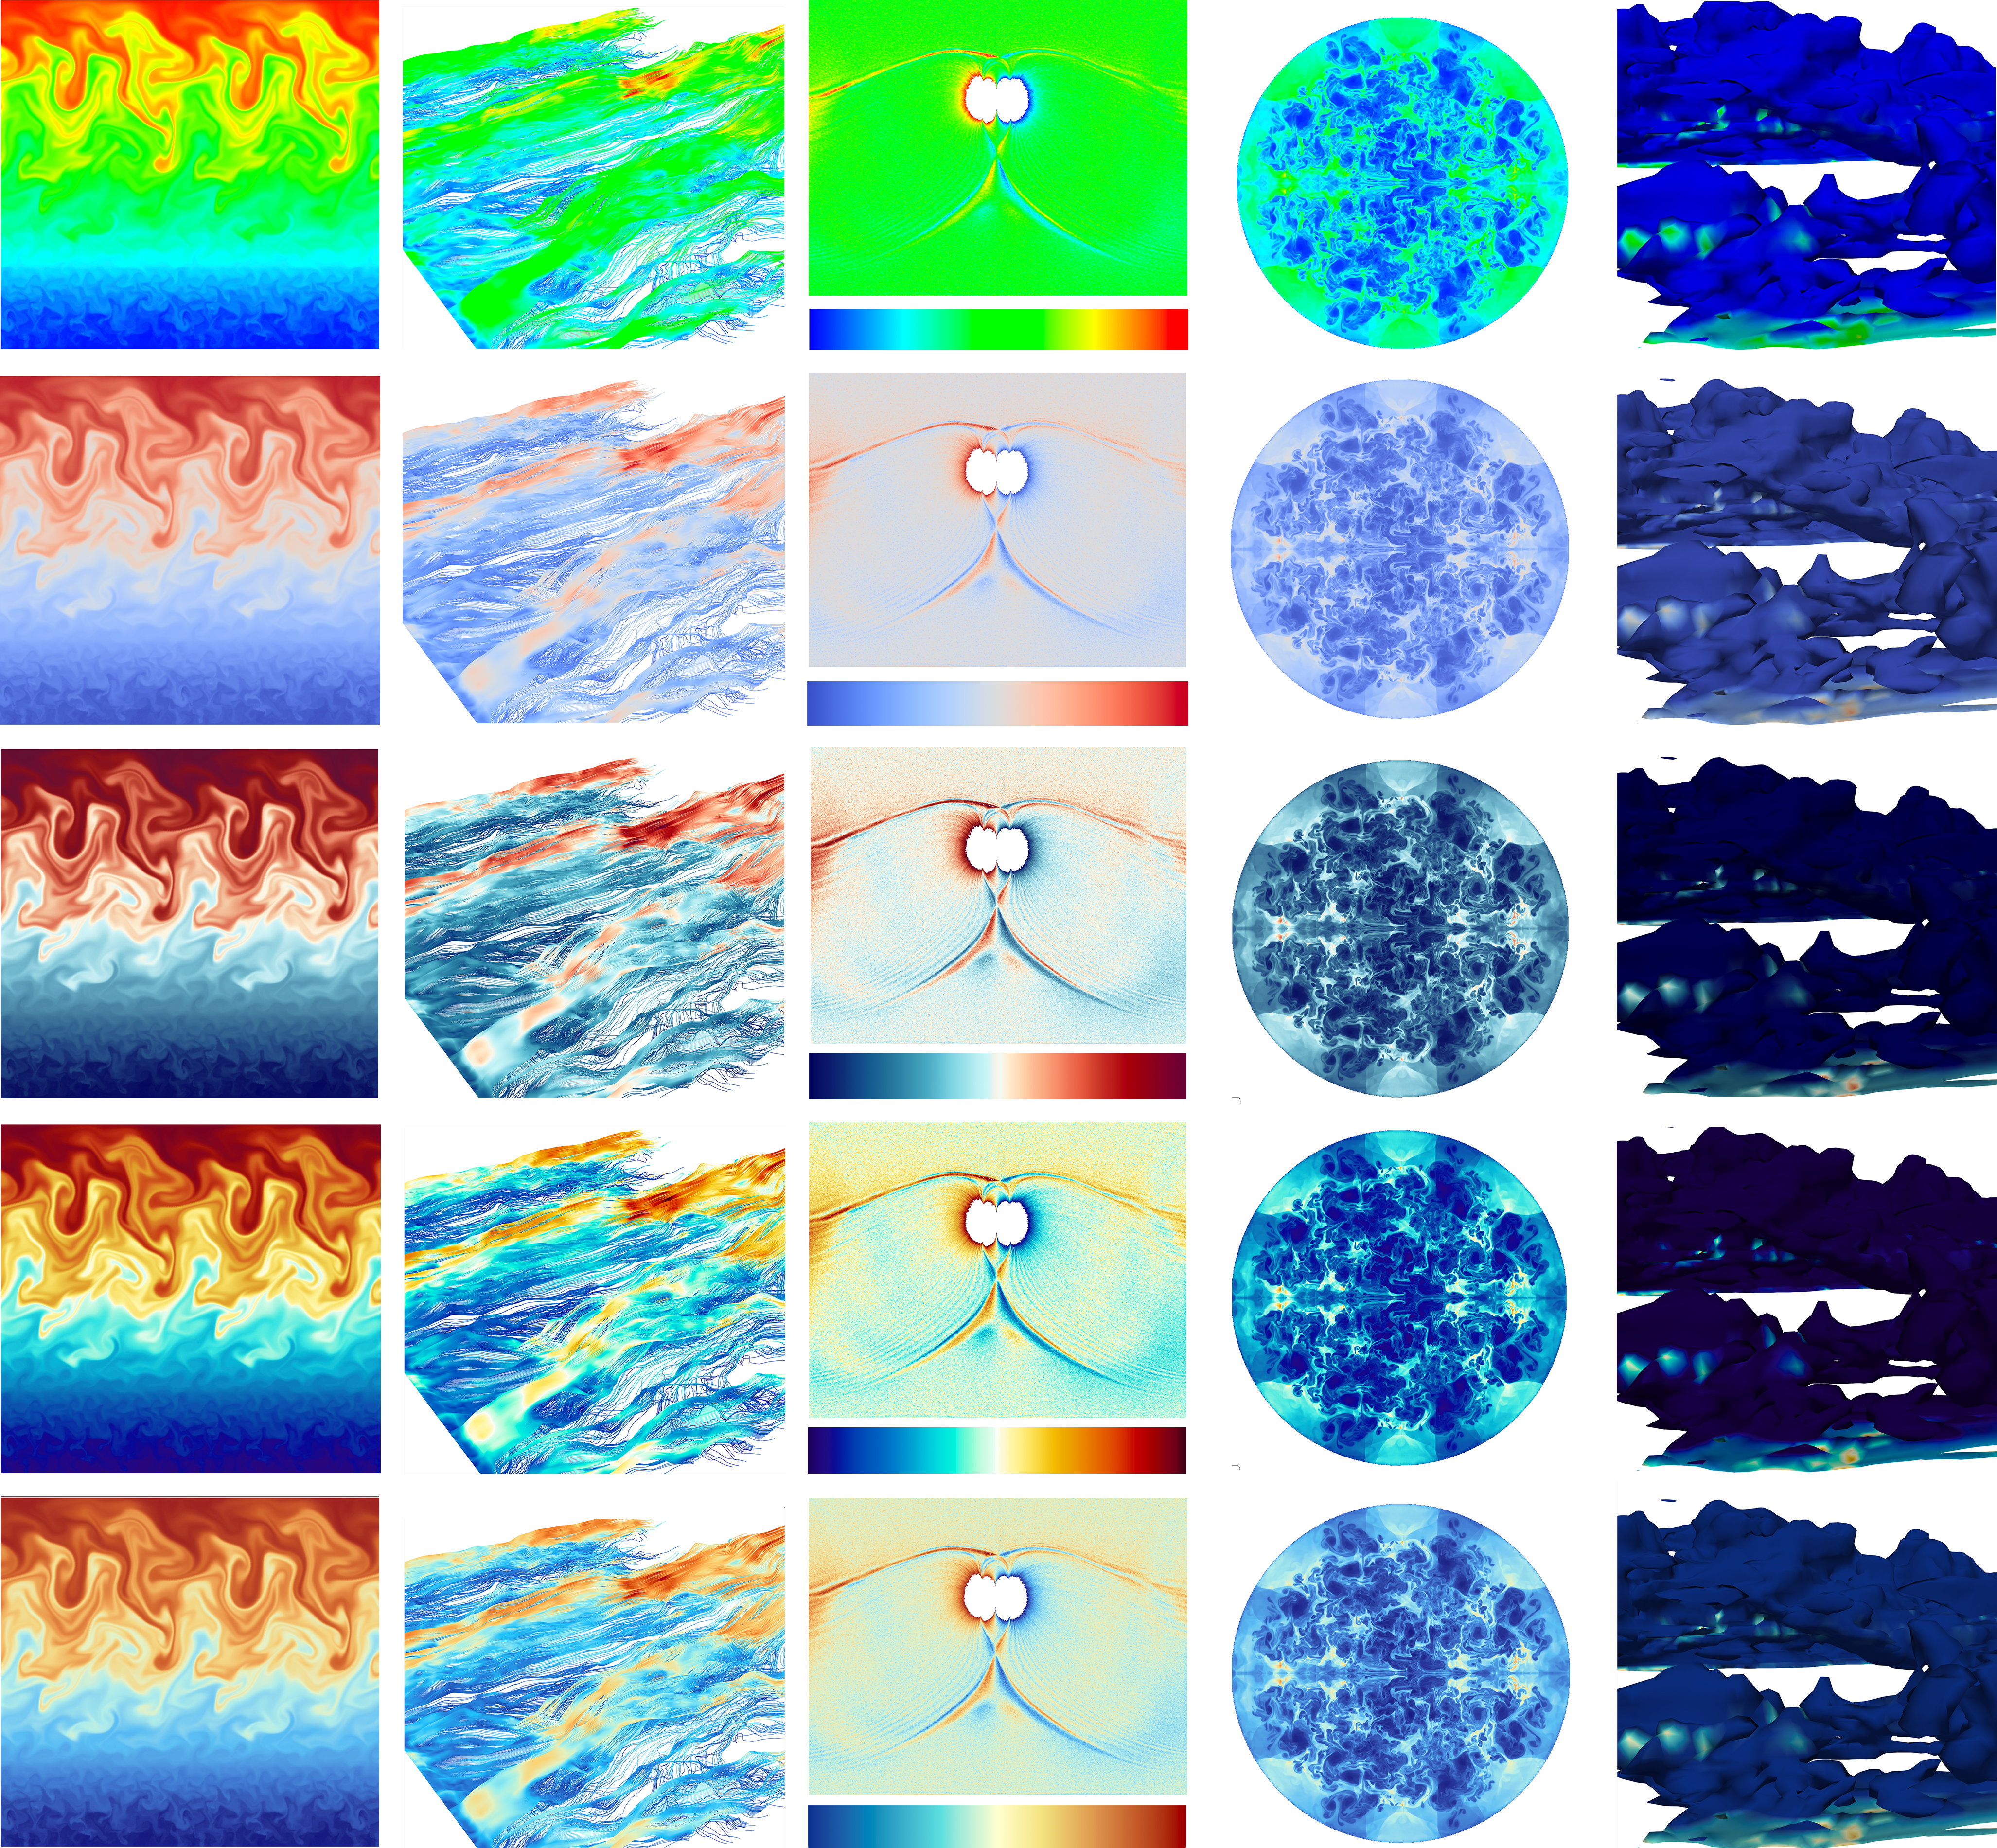
\includegraphics[width=\textwidth]{TheMatrix}
\caption{\DIFaddFL{Left to right are five datasets: ocean kinetic energy; wildfire wind; magnetic reconnection; combustion simulation; wildfire smoke. They are organized by the data characteristics: the two left columns contain data spanning the full range, relatively evenly; the middle column is noisy data that spans the full range but is concentrated in the mid-range; the right two columns contain data concentrated on the low end, 2D and 3D, in column four and five respectively. }}
\label{fig:Matrix}
\end{figure*}


\DIFadd{Next}\DIFaddend , we sought to further smooth the center range as well as experiment with lightening the end values to address the shading concerns\DIFdelbegin \DIFdel{shown in Figure~\ref{fig:3d-shading}}\DIFdelend .
We also added a yellow tint to the center values to prevent bright colors from blending into white backgrounds\DIFdelbegin \DIFdel{as shown in Figure~\ref{fig:middle-point}}\DIFdelend \DIFaddbegin \DIFadd{.
Both changes are shown in the middle of Figure~\ref{fig:iterations}}\DIFaddend .


\DIFdelbegin %DIFDELCMD < \begin{figure}[tb]
%DIFDELCMD < \includegraphics[width=\linewidth]{Final_Pics/white_yellow.png}
%DIFDELCMD < %%%
%DIFDELCMD < \caption{%
{%DIFAUXCMD
\DIFdelFL{Wind streamlines using our first iteration of }%DIFDELCMD < \fast %%%
\DIFdelFL{containing a white center value and the final version of }%DIFDELCMD < \fast %%%
\DIFdelFL{with saturation increased in the mid-range.}}
%DIFAUXCMD
%DIFDELCMD < \label{fig:middle-point}
%DIFDELCMD < \end{figure}
%DIFDELCMD < 

%DIFDELCMD < \begin{figure*}[htb]
%DIFDELCMD <   \centering
%DIFDELCMD <   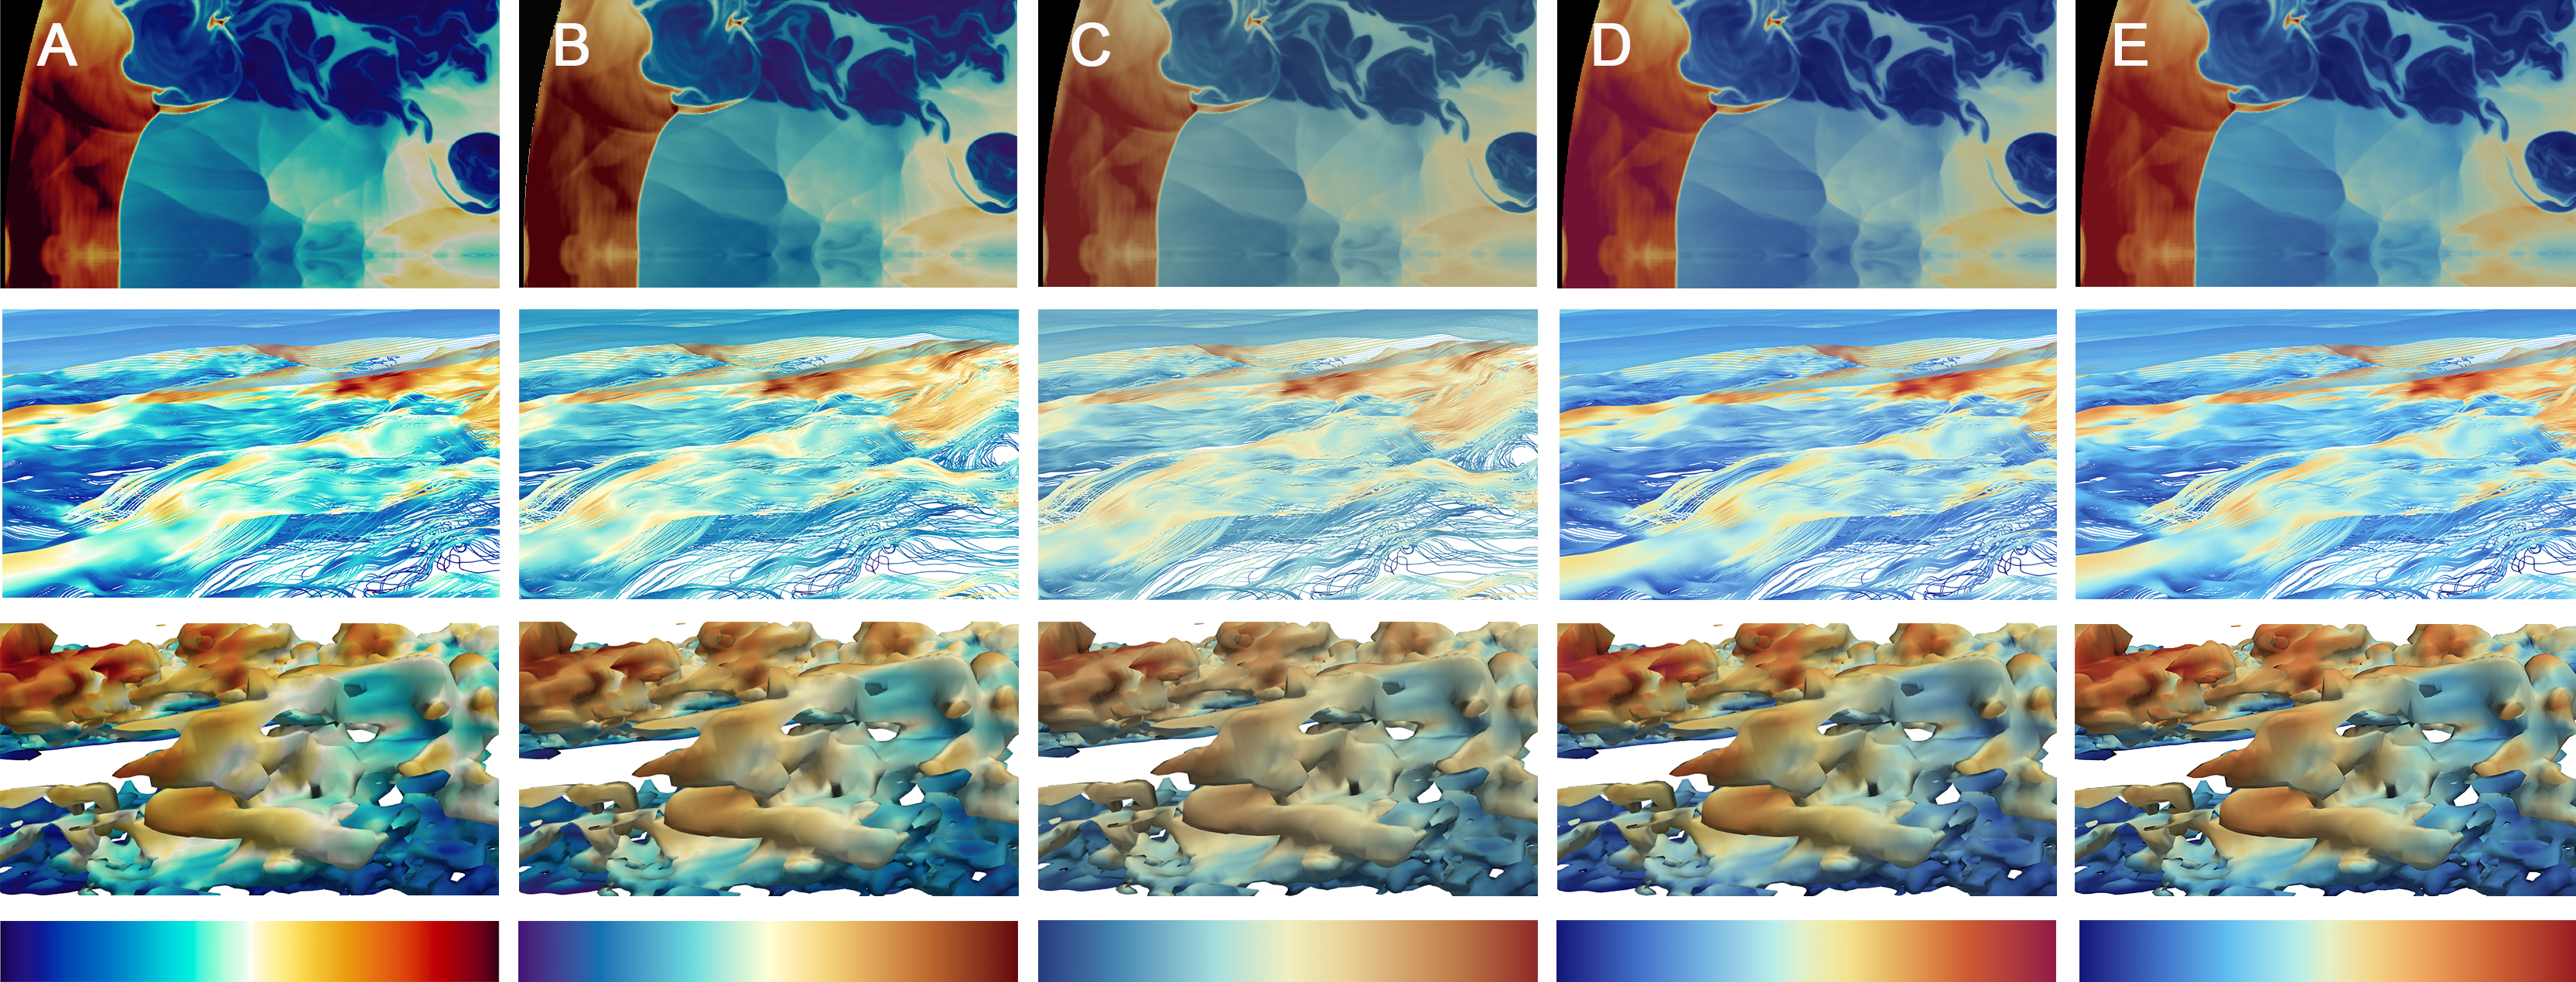
\includegraphics[width=\textwidth]{Final_Pics/Iterative5letters.png}
%DIFDELCMD <   %%%
%DIFDELCMD < \caption{%
{%DIFAUXCMD
\DIFdelFL{Iterative design from the }%DIFDELCMD < \blueorange %%%
\DIFdelFL{colormap (A) to our final design of }%DIFDELCMD < \fast %%%
\DIFdelFL{(E).
    The impact of each iteration is demonstrated on three types of data: 2D continuous combustion data (LLNL), streamlines of wind from a fire simulation (LANL), and volumetric data of smoke from the same fire simulation.
    %DIF < \fix{The prose refers to columns labeled A--E, but no such labels are in the figure. --Ken}
  }}
%DIFAUXCMD
%DIFDELCMD < \label{fig:iterations}
%DIFDELCMD < \end{figure*}
%DIFDELCMD < 

%DIFDELCMD < %%%
\DIFdelend However, the discriminatory power of this colormap was significantly compromised from these previous changes. \DIFdelbegin \DIFdel{In response, we increased }\DIFdelend \DIFaddbegin \DIFadd{We tried increasing }\DIFaddend the saturation across the colormap and \DIFdelbegin \DIFdel{extended }\DIFdelend \DIFaddbegin \DIFadd{extending }\DIFaddend the warm hues toward purple\DIFdelbegin \DIFdel{for the iteration in column D. This map was close but our evaluation methods showed lower discriminability in the center ranges. }%DIFDELCMD < 

%DIFDELCMD < %%%
\DIFdelend \DIFaddbegin \DIFadd{. Here the transition toward fushsia became problematic. }\DIFaddend To compensate, we increased the saturation again\DIFaddbegin \DIFadd{, removed the purple }\DIFaddend and shifted the turquoise region toward the center to provide \DIFdelbegin \DIFdel{extra discriminationin this region}\DIFdelend \DIFaddbegin \DIFadd{the needed discrimination}\DIFaddend , resulting in the final \fast colormap shown \DIFdelbegin \DIFdel{in column E.
This subtle increase in detail is visible in the 2D data }\DIFdelend \DIFaddbegin \DIFadd{on the right }\DIFaddend of Figure~\ref{fig:iterations}\DIFdelbegin \DIFdel{while still maintaining a good middle point and 3D shading behavior}\DIFdelend .

%DIF < \fix{I removed a reference to Figure~\ref{fig:designs}, suggesting that those were the maps with candidates. As I recall, the refinement was pertubations of Figure~\ref{fig:design:iteration2} only. We used to have a figure for that. It got removed, but that's probably OK. (Ken)}
These candidate colormaps manifest different balances of our criteria: the luminance range to balance discriminability and 3D shading, different luminance adjustments at the \DIFdelbegin \DIFdel{centerpoint }\DIFdelend \DIFaddbegin \DIFadd{center point }\DIFaddend to balance uniformity and smoothness, \DIFaddbegin \DIFadd{and }\DIFaddend different hue ranges to balance discriminability and order.


%DIF < Figure \ref{fig:iterations} illustrates the process of balancing maximum discriminatory power, uniformity and smoothness while maintaining robustness to 3D shading and colorblindness. Specifically, the changes made from left to right are: our starting point, blue-orange divergent; aiming for smooth uniform transitions across the colormap; further smoothing of the center range; increasing the discriminatory power by expanding both the value and saturation range across the colormap; maintaining the discriminatiory power at in the middle range as well as unifying and smoothing the transitions by shifting the hue distributions.
%DIF > %\centering
%DIF > \includegraphics [width=\textwidth]{Final_Pics/Shadow_lights_H.png}
%DIF > \caption{Left to right, \coolwarm, \coolwarm with light added, \fast, \fast with light added.}
%DIF >  \label{fig:3d-shading}
%DIF > \end{figure*}

\DIFdelbegin \DIFdel{Figure \ref{fig:iterations} illustrates the applications of these candidate colormapsto three types of data - continuous 2D data, streamlines, }\DIFdelend \DIFaddbegin \DIFadd{Colormaps for 3D surfaces have an added complexity.
3D forms are principally defined by shading, but the brightness of a colormap can interfere with the interpretation of shading.
%DIF > Figure~\ref{fig:Matrix}, right column, illustrates the issue.
%DIF > In the mid-value range of the colormap they shift the value but do not disrupt our ability to see the forms.
%DIF > In the low and high ends of the colormap, where the hues are the dark, shadows can prevent us from seeing the shape altogether.
%DIF > Given that luminance is the most powerful contrast type, the sacrifice is significant.
%DIF > Figure~\ref{fig:ware} details the impact on the discriminatory power.
The right column in Figure~\ref{fig:Matrix} illustrates the interference of shading and colors in }\coolwarm\DIFadd{, }\blueorange\DIFadd{, }\fast\DIFadd{, and other colormaps.
}\coolwarm\DIFadd{, second row, addresses this issue by not including darker blues and reds, but it does so at a cost of lowering the discriminatory power.
%DIF > In the \coolwarm the 3D forms are clearer than but in visualizations showing the full range of the data, detail is lost.
In contrast, the }\extendedcoolwarm \DIFaddend and \DIFdelbegin \DIFdel{volumetric data.
}\DIFdelend \DIFaddbegin \blueorange \DIFadd{colormaps, third and fourth rows, have colors dark enough to completely hide the shape of objects they are applied to.
As a compromise, }\fast \DIFadd{employs a wider span of the luminance range than }\coolwarm \DIFadd{but less than }\extendedcoolwarm \DIFadd{or }\blueorange\DIFadd{.
%DIF > When using \fast, one can add a default light under the light inspector function, requiring only a box check, a much easier task than trying to increase the internal luminance range as that would require adding and adjusting individual control points.
}\DIFaddend 


%DIF < Some colormaps performed slightly better on specific types of data: streamlines; volumes; 2D surfaces and point data.
%DIF < The differences aligned with the density of the data and the background color.
%DIF < Using this information, the team balanced the considerations between the types of data, user preferences and characteristics of the colormaps.
\DIFdelbegin %DIFDELCMD < 

%DIFDELCMD < %%%
%DIF < Once the colors of the map were agreed on, we made final adjustments for smoothness, uniformity, and discriminatory power.
\DIFdelend Finally, a sequence of control points was chosen for a piecewise-linear interpolation of colors in CIELAB space with a preference to minimize their number.
In practice, users sometimes wish to modify a colormap to their purpose.
For example, users may wish to adjust the colors to highlight particular regions of their scalar data.
This cannot be done easily with larger numbers of control points, so we removed any control points where interpolation produces nearly identical results.
Our final design has nine control points as it is the minimum needed to produce a smoothly transitioning map that moves through the hues we have selected.



%DIF < % \begin{figure}
%DIF < % \centerline{\includegraphics[width=18.5 pc]{pics/Charts.png}}
%DIF < % \caption{Colormap properties displayed in CCC Tool \cite{Nardini2021} for \coolwarm and \fast.}
%DIF < % \label{Charts}
%DIF < % \end{figure}
\DIFdelbegin %DIFDELCMD < 

%DIFDELCMD < %%%
\DIFdelend \section{USER FEEDBACK}

%DIF <  Commenting out these two paragraphs. They cover the same ground as the last two paragraphs of the previous section, and neither has anything to do with user feedback.
\DIFdelbegin %DIFDELCMD < 

%DIFDELCMD < %%%
%DIF < % This initial set of colormaps spawned a discussion among the ParaView development team and produced some mild opinions. These were used to cull down to three sets of maps that varied by: the luminance level, (darkness), at the ends of the colormap; the saturation levels across the colormap; and the smoothness and value of the center transition from cool to warm. All these colormap variations considered retained their perceptual uniformity and robustness to colorblindness.
%DIFDELCMD < 

%DIFDELCMD < %%%
%DIF < % Once the colors of the map were agreed on, the team optimized the colors for smoothness and adjusted colors for equal distribution of discriminatory power.
%DIF < % We decided on nine control points as it was the minimum needed to produce a smoothly transitioning map that moves through hues.
%DIF < % See Figure \ref{Charts}.
%DIF < % In practice, users sometimes wish to modify a colormap to their purpose.
%DIF < % For example, users may wish to adjust the colors to highlight particular regions of their scalar data.
%DIF < % This cannot be done easily with larger numbers of control points, so we removed any control points where interpolation in CIELAB space produced similar results.
%DIFDELCMD < 

%DIFDELCMD < %%%
\DIFdelend As we neared completion of the new colormap design, the development team wanted feedback from current users about these changes before being affected by them.
Sandia National Laboratories has a strong ParaView user base and an active support team for them.
The ParaView support team sent an email to the Sandia ParaView users informing them of planned changes and welcoming any feedback.
\DIFaddbegin \DIFadd{The email elicited feedback with the following open-ended text: ``The ParaView team is debating changing the default, as shown below. Note that users can always change back to our current map and palette. If anyone has any opinions on changes, please send your thoughts back to us.''
This was followed by a set of images comparing the }\coolwarm \DIFadd{colormap and an early version of }\fast \DIFadd{along with a potential change in background shade that was being considered.
}\DIFaddend 

Of the roughly 800 users receiving the email, 18 responded back with comments about the change of the default colormap from Cool to Warm to Fast.
Of these, 15 expressed a clear preference for the new colormap.
\DIFdelbegin \DIFdel{Only 1 preferred the original Cool to Warm colormapwith the remaining }\DIFdelend \DIFaddbegin \DIFadd{We made no attempt to quantify the rating of responses, but they ranged from very favorable (e.g., ``I’ll emphatically vote for the neutral gray background and FAST colormap.'' and ``I like the FAST colormap. Seems like it uses more of the color spectrum whereas the other only uses red, white, blue.'') whereas others only had a slight preference (e.g., ``I don’t have a strong opinion on the default color map; I would maybe lean towards the new one.'' and ``The new one does look a bit better, but the old one isn’t too bad either.'').
}

\DIFadd{Of the remaining 3 respondees, }\DIFaddend 2 \DIFdelbegin \DIFdel{expressing no preference}\DIFdelend \DIFaddbegin \DIFadd{did not express a strong preference.
One stated, ``The new/proposed color map seems fine, the minima/maxima seem a little dark to me personally.''
One respondee disapproved of any change but also would use neither colormap: ``I would never vote to change something that is working.  I also never ever use the default color map. I vote do not change.''
Only one respondee gave a preference to the }\coolwarm \DIFadd{colormap citing issues with banding on some displays: ``The one thing I’ll point out is that in the attached image, there appears to be more banding of colors resulting in sharper steps visually (particularly in the bottom half of the image). Probably this is just an artifact, but aside from the increased contrast, it makes me prefer the images }[\DIFaddend of \DIFdelbegin \DIFdel{one over the other. }\DIFdelend \DIFaddbegin \coolwarm{}] \DIFadd{to the ones }[\DIFadd{of }\fast{}]\DIFadd{.''
}

\DIFaddend Although no formal study has been done, we see this \DIFaddbegin \DIFadd{overall }\DIFaddend as a clear general preference \DIFdelbegin \DIFdel{to }\DIFdelend \DIFaddbegin \DIFadd{for }\DIFaddend the new colormap.


\DIFdelbegin %DIFDELCMD < \begin{figure*}[htb]
%DIFDELCMD <   \centering
%DIFDELCMD <   \includegraphics[width=.49\textwidth]{Final_Pics/chart_CW.png}
%DIFDELCMD <   \includegraphics[width=.49\textwidth]{Final_Pics/chart_Fast.png}
%DIFDELCMD <   %%%
%DIFDELCMD < \caption{%
{%DIFAUXCMD
\DIFdelFL{Colormap properties displayed in CCC Tool \mbox{%DIFAUXCMD
\cite{Nardini2021} }\hskip0pt%DIFAUXCMD
for }%DIFDELCMD < \coolwarm %%%
\DIFdelFL{(left) and }%DIFDELCMD < \fast %%%
\DIFdelFL{(right).}}
  %DIFAUXCMD
%DIFDELCMD < \label{Charts}
%DIFDELCMD < \end{figure*}
%DIFDELCMD < 

%DIFDELCMD < %%%
\DIFdelend \section{PERCEPTUAL EVALUATION}

Although we have not yet had a chance to perform formal human subject studies, we are confident that \fast will outperform its predecessor, \coolwarm, in terms of discriminability.
In particular, \fast has a higher $\Delta$E discriminability metric.
As measured by \DIFdelbegin \DIFdel{CCC Tool}\DIFdelend \DIFaddbegin \DIFadd{CCC-Tool}\DIFaddend ~\cite{Nardini2021}, \coolwarm has an average local CIE$\Delta$E2000 discriminability score of 120 whereas \fast has a score of \DIFdelbegin \DIFdel{174, and the other }\DIFdelend \DIFaddbegin \DIFadd{174. Other }\DIFaddend discriminability metrics similarly show improvements with \fast.
All that said, we recognize that \fast%
%DIF < , shown in Figure \ref{Ast},
%DIF > , shown in Figure \ref{Larsen3},
likely performs less well \DIFdelbegin \DIFdel{in general }\DIFdelend \DIFaddbegin \DIFadd{with respect to discriminability }\DIFaddend than the \blueorange colormap it is based on \DIFdelbegin \DIFdel{.
This is out of necessity }\DIFdelend \DIFaddbegin \DIFadd{as }\blueorange \DIFadd{includes a larger luminence range, being darker on the ends and going to white in the center.
These changes were necessary in order }\DIFaddend to adjust for the smoothness and robustness to shading on 3D surfaces.

The \coolwarm colormap was designed about 15 years ago to move away from the \huewheel colormap and its rainbow colors because of the strong evidence at the time of its poor perceptual properties~\cite{Rogowitz1998,Borland2007,Ware1988,Light2004}.
In the interim, multiple colormaps based on the hues of the rainbow that correct some of the problems of the \huewheel have been designed.
More recent research suggests that added hues and more nameable colors can assist in color differentiations that are not otherwise explained by our perceptual color models \cite{Reda2021}.
This leads some to suggest that perceptually correct colormaps based on rainbow colormaps might be favorable \cite{Ware2023}.
Although the \fast colormap does not incorporate all rainbow hues, it does improve dramatically over the hues provided by \coolwarm\DIFdelbegin \DIFdel{as seen in the hue plots of Figure~\ref{Charts}}\DIFdelend .

\fast also has more namable colors than its \coolwarm predecessor.
Using the color categorization tendency metric proposed by Reda \cite{Reda2022}, \fast once again exceeds \coolwarm.
Using a color name similarity threshold of 0.6 (as was used by Reda), \coolwarm has a categorization tendency metric of 310 whereas \fast scores 369.
That said, \fast could likely be improved further by completing the rainbow with distinctive green hues (much like the \turbo colormap~\cite{Mikhailov2019} does).
However, these are all recent observations deserving more study, particularly for effects beyond discriminability.
Thus, we are not ready to loop back around to the full hues of a rainbow.


\section{CONCLUSION}

Our final iteration of the new colormap, which we dub ``\fast,''\DIFaddbegin \footnote{\DIFadd{The name }\fast \DIFadd{is meaningless, but was chosen as it is reminiscent of other colormap names like }\colormap{Jet} \DIFadd{and }\turbo\DIFadd{.}} \DIFaddend is demonstrated in Figure~\DIFdelbegin \DIFdel{\ref{Ast} }\DIFdelend \DIFaddbegin \DIFadd{\ref{Larsen3} }\DIFaddend as well as numerous other figures in this paper.
\DIFaddbegin \DIFadd{The colors are listed in Table~\ref{tab:colors}.
}\DIFaddend This colormap is provided as one of the available colormaps in ParaView~5.12 and will become the default colormap in ParaView~5.13.

\DIFaddbegin \definecolor{fast0}{RGB}{ 14,  14, 120}
\definecolor{fast1}{RGB}{ 62, 117, 207}
\definecolor{fast2}{RGB}{ 91, 190, 243}
\definecolor{fast3}{RGB}{175, 237, 234}
\definecolor{fast4}{RGB}{229, 241, 196}
\definecolor{fast5}{RGB}{244, 213, 130}
\definecolor{fast6}{RGB}{237, 158,  80}
\definecolor{fast7}{RGB}{204,  90,  41}
\definecolor{fast8}{RGB}{150,  20,  30}

\newcommand*{\colordemo}[1]{\colorbox{#1}{\phantom{X}}}

\begin{table}[t]
  \centering
  \caption{
    \DIFaddFL{Color values used for the }\fast \DIFaddFL{colormap control points.
    These colors are intended to be interpolated in the CIELAB color space.
    Note that these control points are not evenly distributed.
    Pay mind to the interpolant x.
  }}
  \label{tab:colors}
  %DIF > % \begin{tabular}{r@{\quad~( }r@{, }r@{, }r@{ )\quad~( }r@{, }r@{, }r@{ )\quad~}c}
  %DIF > %   \toprule
  %DIF > %   \multicolumn{1}{c@{\quad~\phantom{( }}}{x} & \multicolumn{3}{c@{\phantom{ )}\quad~\phantom{( }}}{RGB} & \multicolumn{3}{c@{ \phantom{)}\quad~}}{CIELAB} \\
  %DIF > %   \midrule
  %DIF > %   0.00 &  14 &  14 & 120 &   14.3 &  39.5 & -57.3 & \colordemo{fast0} \\
  %DIF > %   0.17 &  62 & 117 & 207 &   49.9 &  11.4 & -51.5 & \colordemo{fast1} \\
  %DIF > %   0.30 &  91 & 190 & 243 &   73.2 & -13.3 & -35.1 & \colordemo{fast2} \\
  %DIF > %   0.43 & 175 & 237 & 234 &   89.7 & -19.9 &  -4.8 & \colordemo{fast3} \\
  %DIF > %   0.50 & 229 & 241 & 196 &   93.2 & -11.3 &  20.4 & \colordemo{fast4} \\
  %DIF > %   0.59 & 244 & 213 & 130 &   86.1 &   0.4 &  44.8 & \colordemo{fast5} \\
  %DIF > %   0.71 & 237 & 158 &  80 &   71.6 &  21.9 &  51.5 & \colordemo{fast6} \\
  %DIF > %   0.85 & 204 &  90 &  41 &   52.1 &  42.6 &  48.5 & \colordemo{fast7} \\
  %DIF > %   1.00 & 150 &  20 &  30 &   32.0 &  51.4 &  30.6 & \colordemo{fast8} \\
  %DIF > %   \bottomrule
  %DIF > % \end{tabular}
  \begin{tabular}{r@{\quad~( }r@{, }r@{, }r@{ )\quad~}c@{}c}
    \toprule
    \multicolumn{1}{c@{\quad~\phantom{( }}}{x} & \multicolumn{3}{c@{\phantom{ )}\quad~\phantom{( }}}{RGB} & \multicolumn{2}{c}{Color} \\
    \midrule
    \DIFaddFL{1.00 }& \DIFaddFL{150 }&  \DIFaddFL{20 }&  \DIFaddFL{30 }& \colordemo{fast8} & \multirow{9}{.26 in}{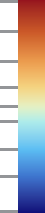
\includegraphics{fast-colorbar-vertical}} \\
    \DIFaddFL{0.85 }& \DIFaddFL{204 }&  \DIFaddFL{90 }&  \DIFaddFL{41 }& \colordemo{fast7} \\
    \DIFaddFL{0.71 }& \DIFaddFL{237 }& \DIFaddFL{158 }&  \DIFaddFL{80 }& \colordemo{fast6} \\
    \DIFaddFL{0.59 }& \DIFaddFL{244 }& \DIFaddFL{213 }& \DIFaddFL{130 }& \colordemo{fast5} \\
    \DIFaddFL{0.50 }& \DIFaddFL{229 }& \DIFaddFL{241 }& \DIFaddFL{196 }& \colordemo{fast4} \\
    \DIFaddFL{0.43 }& \DIFaddFL{175 }& \DIFaddFL{237 }& \DIFaddFL{234 }& \colordemo{fast3} \\
    \DIFaddFL{0.30 }&  \DIFaddFL{91 }& \DIFaddFL{190 }& \DIFaddFL{243 }& \colordemo{fast2} \\
    \DIFaddFL{0.17 }&  \DIFaddFL{62 }& \DIFaddFL{117 }& \DIFaddFL{207 }& \colordemo{fast1} \\
    \DIFaddFL{0.00 }&  \DIFaddFL{14 }&  \DIFaddFL{14 }& \DIFaddFL{120 }& \colordemo{fast0} \\
    \bottomrule
  \end{tabular}
\end{table}

\DIFaddend Revisiting the criteria presented at the beginning of this paper, \DIFdelbegin \DIFdel{we feel there is a clear advantage of the new colormap}\DIFdelend \DIFaddbegin \DIFadd{evaluations and user feedback show the advantages of }\fast \DIFadd{over }\coolwarm \DIFadd{and other standard defaults. Figure~\ref{fig:Matrix} provides comparisons of the criteria across five data sets}\DIFaddend .



\DIFdelbegin %DIFDELCMD < \begin{figure}
%DIFDELCMD < \includegraphics[width=\linewidth]{pics/Larsen2.png}
%DIFDELCMD < %%%
%DIFDELCMD < \caption{%
{%DIFAUXCMD
\DIFdelFL{Combustion simulation (Larsen, LLNL) of }%DIFDELCMD < \coolwarm %%%
\DIFdelFL{(left) and }%DIFDELCMD < \fast %%%
\DIFdelFL{(right) colormaps demonstrating to discriminatory power in the mid-range of data values.}}
%DIFAUXCMD
%DIFDELCMD < \label{Larsen}
%DIFDELCMD < \end{figure}
%DIFDELCMD < 

%DIFDELCMD < %%%
\DIFdelend \begin{itemize}

\item \emph{Discriminative \DIFdelbegin \DIFdel{powers}\DIFdelend \DIFaddbegin \DIFadd{power}\DIFaddend } --
  \fast performs better on every color discriminability metric that we have available.
\item \emph{Uniformity} --
  The previous \coolwarm colormap has very little luminance change in its center leaving a region of colors that tend to get washed out (see \DIFdelbegin \DIFdel{Figure \ref{Larsen}}\DIFdelend \DIFaddbegin \DIFadd{Figures \ref{Larsen3} and \ref{fig:Matrix}}\DIFaddend ).
  \fast retains more luminance variation at its apex to help maintain a uniform perceptual change in that region.
\item \emph{Smoothness} --
  \fast sacrifices some smoothness at the center for gain in discrimination and uniformity, but the smoothness is close to \coolwarm and much better than \blueorange.
\item \emph{Order} --
  \coolwarm and \fast use the same cues of luminance and warmth for color order.
\item \emph{Robustness to shading on 3D surfaces} --
  \fast allows the end colors to become darker for greater discriminability.
  This makes shapes a bit harder but still possible to discern in the worst case scenario of values all at one end of the colormap range (see Figure~\DIFdelbegin \DIFdel{\ref{fig:3d-shading}).
  }\DIFdelend \DIFaddbegin \DIFadd{\ref{fig:Matrix}, right column).
  Although dark surfaces can be reveled with brighter lighting, such bright colors could wash out light colors.
  Requiring customized lighting is just pushing the problem back on the user again, so we discount this solution.
  It is also conceivable that changes in lightness could obfuscate the shape.
  Research for such an effect is lacking, but anecdotally we have not encountered such an occurrence.
}\DIFaddend \item \emph{Robustness to colorblindness} --
  Colorblindness was always kept in mind when designing \fast.
  Figure~\ref{fig:colorblindness} shows that \fast responds just as well to common forms of colorblindness as does \coolwarm.
\item \emph{Aesthetically pleasing} --
  Aesthetics are notoriously difficult to measure with any accuracy.
  However, voluntary responses from ParaView users suggest a preference for \fast.

\end{itemize}



With the introduction of \fast as the default colormap for ParaView, we make a significant improvement in the readability of colors in many visualizations produced. We are proud to have the opportunity to have such a broad impact on the scientific community. \DIFaddbegin \fast \DIFadd{can be downloaded at: }\url{https://sites.utexas.edu/artscivis/color/} \DIFadd{or }\url{https://www.kennethmoreland.com/color-advice/}\DIFadd{.
}\DIFaddend 

\begin{figure}[htb]
  \centering
  \begin{tabular}{cc}
    \includegraphics[width=.44\linewidth, height=5mm]{map-cool-to-warm} & \includegraphics[width=.44\linewidth, height=5mm]{map-fast} \\
    \includegraphics[width=.44\linewidth, height=5mm]{map-protanopia-cool-to-warm} & \includegraphics[width=.44\linewidth, height=5mm]{map-protanopia-fast} \\
    \includegraphics[width=.44\linewidth, height=5mm]{map-deurteranopia-cool-to-warm} & \includegraphics[width=.44\linewidth, height=5mm]{map-deurteranopia-fast}
  \end{tabular}
  \caption{
    Colorblindness simulation of \coolwarm (left) and \fast (right) colormaps.
    The top row is the original colors.
    The middle row is the colors simulated for protanopia.
    The bottom row is the colors simulated for deurteranopia.
  }
  \label{fig:colorblindness}
\end{figure}

\section{ACKNOWLEDGMENT}

The authors wish to thank the ParaView software development team at Kitware, Inc. for assisting in making these changes to the software. We also wish to thank those in the ParaView community who provided the necessary feedback to guide our designs. We also wish to acknowledge the contributions made by the Data Science at Scale, LANL~\cite{SciVisColor}, for their contributions and support for the underlying color research and Khairi Reda for help with namability evaluations of colormaps.

This work was supported in part by the U.S. Department of Energy (DOE) RAPIDS SciDAC project under contract number DE-AC05-00OR22725. This paper describes objective technical results and analysis. Any subjective views or opinions that might be expressed in the paper do not necessarily represent the views of the U.S. Department of Energy or the United States Government. This work was done in part at Sandia National Laboratories, which is a multi-mission laboratory managed and operated by National Technology and Engineering Solutions of Sandia, LLC, a wholly owned subsidiary of Honeywell International Inc., for the U.S. Department of Energy's National Nuclear Security Administration under contract DE-NA0003525.

\DIFaddbegin \DIFadd{We would like to thank all of the scientists who lent their data and provided feedback on the colormaps. The data was provided by scientists at US DOE Laboratories including: M. Petersen, MPAS-Ocean, LANL; R. Linn, LANL, wildfire; W. Daughton, LANL, magnetic reconnection; M. Larsen, LLNL, combustion simulation.
}


\DIFaddend \bibliographystyle{IEEEtran}
\bibliography{Fast_ParaView}

\begin{IEEEbiography}{Francesca Samsel}{\,} is a \DIFdelbegin \DIFdel{Research Scientist at the }\DIFdelend \DIFaddbegin \DIFadd{research scientist in the Visualization Group at The }\DIFaddend Texas Advanced Computing Center, University of Texas at Austin. She received an M.F.A. from the University of Washington and a B.F.A. from California College of Art. Prior to turning her attention to scientific visualization she taught sculpture and design in the Art Department of Fordham University at Marymount. Her research focuses on expanding the visual language used to encode scientific data\DIFaddbegin \DIFadd{, which started with her work on color, }\DIFaddend as well as experimenting with forms of interactive and physicalized data. Contact her at fsamsel@tacc.utexas.edu.
\end{IEEEbiography}

\begin{IEEEbiography}{W. Alan Scott}{\,}is Sandia National Laboratories' ParaView Support Manager.  He received an MS degree in computer science from Utah State University in 1992, focusing on computer architectures, parallel processing, compiler design, and graphics.  His current interests include ParaView functionality and user experiences.  Contact him at wascott@sandia.gov.
\end{IEEEbiography}

\begin{IEEEbiography}{Kenneth Moreland,}{\,} with Oak Ridge National Laboratory, is a senior member of IEEE.
  He received MS and Ph.D. degrees in computer science from the University of New Mexico in 2000 and 2004, respectively.
  Dr. Moreland specializes in large-scale visualization and graphics and plays an active role in the development of several HPC products including ParaView, VTK, IceT, Catalyst, and VTK-m.
  His current interests include the design and development of visualization algorithms and systems to run on multi-core, many-core, and future-generation computer hardware.
  Contact him at morelandkd@ornl.gov.
\end{IEEEbiography}

\end{document}

